\documentclass{article}


\usepackage[english]{babel}
\usepackage{listings}

\usepackage[letterpaper,top=2cm,bottom=2cm,left=3cm,right=3cm,marginparwidth=1.75cm]{geometry}

% Useful packages
\usepackage{amsmath}
\usepackage{graphicx}
\usepackage[colorlinks=true, allcolors=blue]{hyperref}
\usepackage{listings}
\lstset{language=Python}

\title{COSC 343: homework 4 Runge-Kutta}
\author{Micah Sherry}

\begin{document}
\maketitle
\section{Lotka-Voltera Model}
For class we looked at the populations of two species, a prey denoted by $y_1$ and a
predator denoted by $y_2$, can be modeled by the autonomous, nonlinear ODE
$$
\bf{y}' =
\begin{pmatrix}
	y_1' \\ y_2'
\end{pmatrix} = 
\begin{pmatrix}
	y_1(\alpha_1-\beta_1y_2) \\ y_2(-\alpha_2+\beta_2y_1)
\end{pmatrix}
= \bf{f(y)}
$$
This model is known as the Lotka-Voltera model. The parameters $\alpha_1$ and $\alpha_2$ are birth
and death rates in isolation for prey and predators respectively. The parameters$\beta_1$ and $\beta_2$ determine the effects of the interactions of the two species. Write a program that
uses the classical fourth order Runge-Kutta method to solve the Lotka-Voltera system.
Integrate from t = 0 to t = 25. For class we will use the parameters $\alpha_1 = 0.5$, $\beta_1 =
0.1$, $\alpha_2 = 1.0$, $\beta_2 = 0.02$, and the initial populations $y_1(0) = 100$, and $y_2(0) = 10$. We
plotted each of the two populations as a function of time, and on a separate graph plot
the trajectory of the point (y1(t), y2(t)) in the plane as a function of time and created
a phase portrait\\
For this assignment try other initial populations. Observe the results using the same
type of graphs used in class. Can you find nonzero initial populations that allow for
either of the populations to become extinct? Can you find a non-zero initial population
that never changes.
\subsection{code:}
\subsubsection*{methods for Runge-Kutta}
\lstinputlisting{../Runge_Kutta.py}
\subsubsection*{methods for Lokta-Voltera}
\lstinputlisting{../Lotka_Voltera.py}



\subsection{initial condition that causes extinction of a population}
consider what would happen as the number of predators approached zero. the growth rate of the prey would look like:
$$y_1' = \alpha_1y_1$$
this tells us that the prey would grow exponentially.
now consider what would happen when the number of prey is going to zero. the death rate of the predators would look like:
$$y_2' = -\alpha_2y_2$$
this tells us that the predators would die exponentially and as I already established when the number predators goes to zero the number of prey grows exponentially. so what this tells us is there no initial condition that will cause one of the populations to go extinct. 
\subsection{stable initial condition}
to find initial conditions such that both populations remain constant. If a population is constant then its derivative is zero. so if we set $\bf{y} =\bf{0} $ then solve the system for $y_1$ and $y_2$
$$
\bf{0} = 
\begin{pmatrix}
	y_1(\alpha_1-\beta_1y_2) \\ y_2(-\alpha_2+\beta_2y_1)
\end{pmatrix}
$$
solving this system yields (ignoring the trivial solution):
$$
y_1 = \frac{\alpha_2}{\beta_2} \text{ and }
y_2 = \frac{\alpha_1}{\beta_1} 
$$ 
for the parameters specified above. that would make:
$$
y_1 = 50 \text{ and }
y_2 = 5 
$$  

\subsection{plots}
\begin{figure}[hbt!]
	\centering
	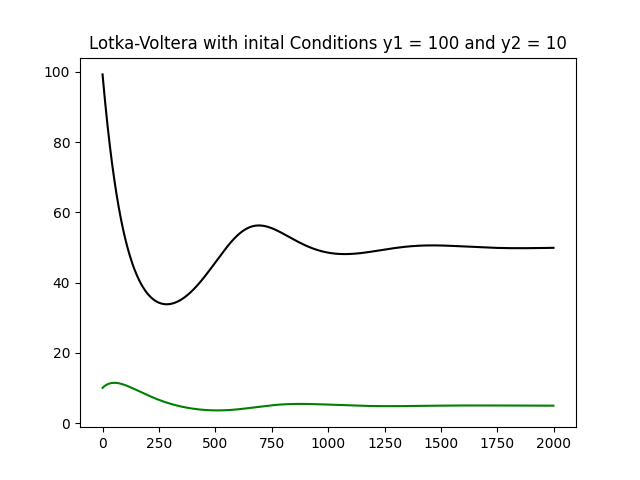
\includegraphics[width=.75\linewidth]{LV_100_10.png}
	
	\label{fig: Lotka-Voltera }
\end{figure}

\begin{figure}[hbt!]
	\centering
	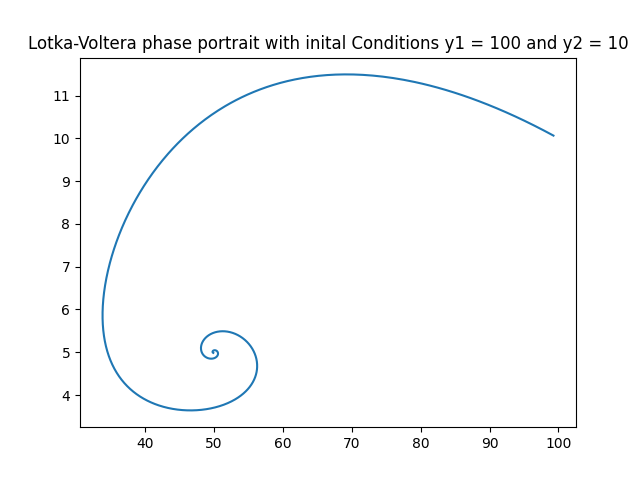
\includegraphics[width=.75\linewidth]{LV_phase_portrait.png}
	
	\label{fig: Lotka voltera phase portrait}
\end{figure}

\pagebreak
\section{Leslie-Gower Model}
Repeat your work using the Leslie-Gower model:
$$
\bf{y}' =
\begin{pmatrix}
	y_1' \\ y_2'
\end{pmatrix} = 
\begin{pmatrix}
	y_1(\alpha_1-\beta_1y_2) \\ y_2(\alpha_2-\frac{\beta_2y_2}{y_1})
\end{pmatrix}
= \bf{f(y)}
$$
use the same parameters given above with the exception of setting $\beta_2 = 10$. How does
the solution differ between the two models?
\subsection{code:}
this code uses the same methods for Runge-Kutta as lokta-voltera the only thing that changes is the forcing function  
\lstinputlisting{../Leslie_Gower.py}
\subsection{initial condition that causes extinction of a population}
for this model i was able to find several that led to the extinction of the predators. typically if i set the ratio (prey to predator) of initial conditions to 1.8 (or less) to 1 . 
\subsection{stable initial condition}
As mentioned while answering this question for the Loktka-Voltera model we need to set its derivative to zero and then solve for $y_1 \text{ and }y_2$
$$
\bf{0} =
\begin{pmatrix}
	y_1(\alpha_1-\beta_1y_2) \\ y_2(\alpha_2-\frac{\beta_2y_2}{y_1})
\end{pmatrix}
$$ 
solving this system yields (ignoring the trivial solution):
$$y_1 = \frac{\beta_2}{\alpha_2}y_2 = \frac{\beta_2}{\alpha_2}\frac{\alpha_1}{\beta_1}\text{ and } y_2 = \frac{\alpha_1}{\beta_1}$$ 
and like with Lotka-Voltera model with the given  parameters  the solution is
$$
y_1 = 50 \text{ and }
y_2 = 5 
$$  
\subsection{plots}
\begin{figure}[hbt!]
	\centering
	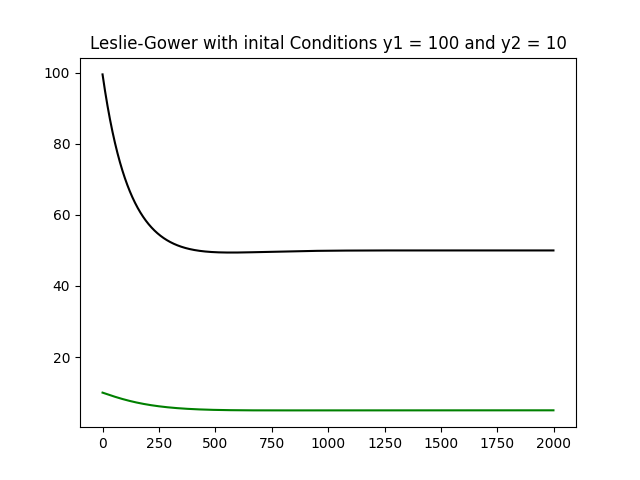
\includegraphics[width=.75\linewidth]{LG_100_10.png}
	
	\label{fig: Leslie Gower }
\end{figure}

\begin{figure}[hbt!]
	\centering
	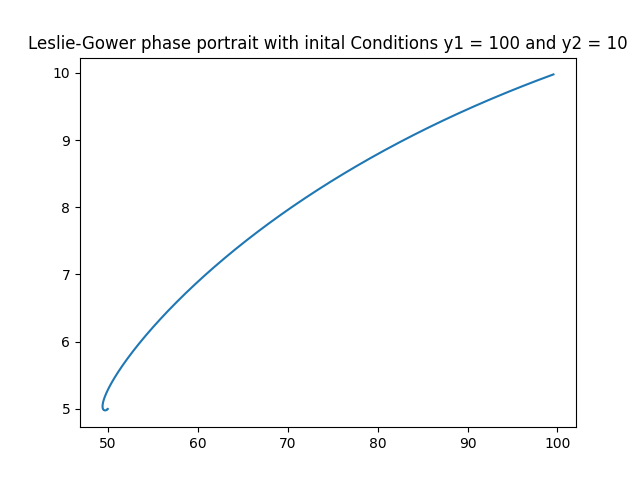
\includegraphics[width=.75\linewidth]{LG_phase_portrait.png}
	
	\label{fig: Leslie Gower Phase portrait}
\end{figure}
\subsection{how do the solutions differ between 2 models}
In the Lokta-Voltera model the populations oscillate more than the Leslie-Gower model. both Models had an initial condition ($y_1 = 50$ and $y_2 = 5$) that caused the populations to remain constant. But only the Leslie-Gower model had an initial condition that will cause extinction.




\end{document}